% replace all text with your own text.
% in this template few examples are mention
\section{Methodology - Model Selection}
\label{sec:method} % Label for method chapter

\subsection{Linear Regression}

Simple linear regression models were applied to explore the association between each type of mental disorder and eating disorders based on standardized data.

The selection of input variables for modeling the prevalence of eating disorders was based on both statistical analysis and the clinical characteristics of each mental disorder in Dataset 1 Prevalence of Mental Illness. In this analysis, we utilized correlation matrices and covariance matrices to evaluate the relationships between the disorders.

% TABLE 1
\begin{table}[h!]
\centering
\textbf{Table 3.1: Correlation}

\begin{tabular}{||p{5cm} c p{8cm}||} 
 \hline
 \textbf{Variable Pair} & \textbf{Correlation (r)} & \textbf{Relationship Strength} \\
 \hline
 bipolar disorders and eating disorders & +0.68 & Strong Correlation \\ 
 \hline
 anxiety disorders and eating disorders & +0.59 & Moderate to Strong Correlation \\
 \hline
 schizophrenia disorders and eating disorders & +0.50 & Moderate Correlation \\
 \hline
 depression disorders and eating disorders & –0.05 & Not Significantly Correlated \\
 \hline
\end{tabular}
\caption{This suggests that bipolar, anxiety, and schizophrenia are positively and significantly correlated with eating disorders, while depression disorders do not appear to be directly related.}
\label{table:3.1}
\end{table}

% TABLE 2
\begin{table}[h!]
\centering
\textbf{Table 3.2: Covariance}

\begin{tabular}{||p{5cm} c p{8cm}||} 
 \hline
 \textbf{Variable Pair} & \textbf{Covariance} & \textbf{Interpretation} \\ 
 \hline
 bipolar and eating disorders & 0.0219 & Increase together, units are quite similar \\ 
 \hline
 anxiety and eating disorders & 0.0864 & Large covariance means change together in larger scales \\
 \hline
 schizophrenia and eating disorders & 0.0027 & Correlation exists, but units of change are significantly different \\
 \hline
\end{tabular}
\caption{Although schizophrenia has a small covariance, it remains significant when combined with other variables in a generalized linear model (GLM) due to its independent effect.}
\label{table:3.2}
\end{table}

We selected three key predictors to build the model: Bipolar disorders, Anxiety disorders, and Schizophrenia disorders. This combination is both statistically robust and reflects clinical utility in predicting eating disorder risk from other psychiatric manifestations.

Next, we used linear regression models to examine the relationship between psychiatric disorders and the prevalence of eating disorders. Both simple linear regression and generalized linear regression (GLM) models in the next section were used to determine the influence and predictive ability of psychiatric factors such as bipolar disorders, anxiety disorders, and schizophrenia disorders.

Using linear regression model:

    \begin{equation}
    \text{Eating Disorders} = \beta_0 + \beta_1 X + \varepsilon
    \end{equation}
    
    Where:
    \begin{itemize}
    \item $X$ is one of three variables: bipolar disorders, anxiety disorders, or schizophrenia disorders
    \item $\beta_0$: is the intercept of the linear regression
    \item $\beta_1$: measures the degree of change in eating disorders as mental disorders change
    \item $\varepsilon$ is the error term, accounting for random variation not explained by the model
    \end{itemize}
    
    \textbf{Results:}
    
    \begin{tabular}{||c c c p{10cm}||} 
    \hline
    \textbf{Predictor} & \textbf{$R^2$} & \textbf{MSE} & \textbf{Interpretation} \\
    \hline
    bipolar disorders &  0.46 & 0.01 & Relatively strong linear relationship. 
    Approximately 46 percent of the variation in eating disorders is explained by bipolar disorders \\ 
    \hline
    anxiety disorders &  0.35 & 0.01 & Moderate relationship. The effect size is smaller than bipolar disorders\\
    \hline
    schizophrenia disorders & 0.25 & 0.01 & Weak to moderate relationship. However, there is a linear increasing trend\\
    \hline
    \end{tabular}

The low MSE (0.01) in all three models indicates that the mean square prediction error is very small, demonstrating that the models have high accuracy in fitting the normalized data.

We performed similar analyses with dataset 2 to support the hypothesis that other psychiatric disorders also have a significant impact on eating disorders. The simple linear regression models revealed a significant positive linear relationship between bipolar disorders and eating disorders, with a correlation coefficient $\ R^2$ of 0.46 and a relatively small mean square error (MSE) of 0.01, indicating a good model fit and well-distributed data. The association between anxiety disorders and eating disorders was also noted at $R^2 = 0.35$, with an MSE of 0.01. In addition, we also observed that bipolar disorders had a moderate relationship with anxiety disorders $R^2 =0.34$, suggesting the possibility that these disorders coexist and influence each other in the same patient group.

\subsubsection{Additional Linear regression}

In addition, we used regression modeling to analyze the connection between healthcare access and depression rates. We performed ordinary least squares (OLS) regression each year to assess the relationship between the UHC index and depression rates during the study period. This method helped us examine both general trends and changes over time in how access to healthcare affects mental health outcomes (\textit{Agresti \& Kateri, 2022}).



\subsubsection{Case Study: Comparison of Sweden and the United States}

This study compares UHC and depression rates in Sweden and the United States. These countries have very different healthcare systems. Sweden has a higher UHC index, which means its healthcare is more accessible, and it also has lower depression rates. In contrast, the U.S. has less coverage and higher depression rates. These findings support earlier studies showing that better access to healthcare leads to better mental health outcomes (World Health Organization, 2023; Patel et al., 2018).

This comparison highlights the importance of accessible and comprehensive healthcare in improving mental health. Sweden’s system emphasizes fair service distribution and preventive care, which appear to enhance mental well-being. In contrast, the U.S. faces persistent gaps in coverage that may exacerbate mental health challenges—especially among vulnerable groups with limited access to care(Prebys Foundation, n.d.)..


% \section{Linear Discriminant Analysis (LDA) - Dylan}

% Linear Discriminant Analysis (LDA) aims to classify two or more classes or categorical variables using the best linear combination of numerical features. LDA maximizes the ratio of variance between-class and the variance within-class. It is interesting to note that this should also provide useful insights into which features should perform best in subsequent clustering model analysis \cite{mclachlan2004discriminant}. 

% In the context of mental health data, we use LDA to classify predefined risk levels (e.g. low, medium, high) of mental disorders based on input variables such as prevalence rates.

% As shown in Figure 3.1, LDA the linear discriminants that enhance the separation of risk groups, thus allowing easier interpretation and predictions.

%     \begin{figure}[!ht]
%         \centering
%         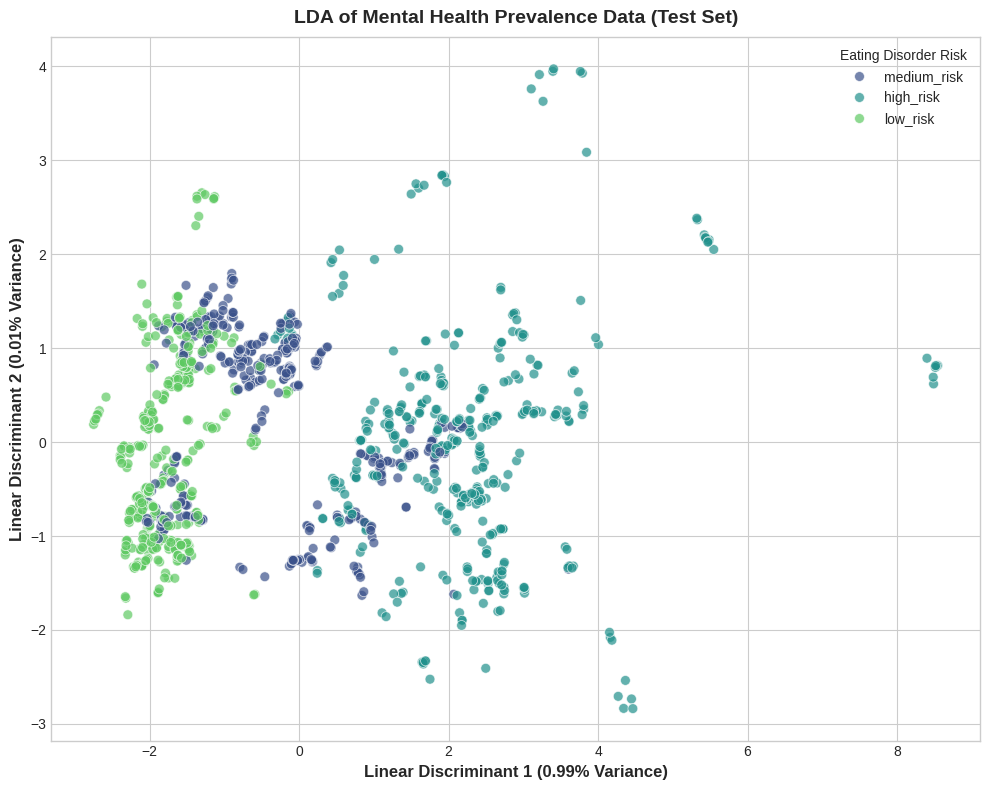
\includegraphics[scale=0.3]{figures/lda_result.png}
%         \caption{LDA}
%         \label{fig:lda}
%     \end{figure}

\section{Predicting prevalence of Eating Orders}

This section covers various prediction models used to predict the rate or prevalence of eating disorders by fitting multiple models to numerical features in the mental illness prevalence dataset [cite]. 

\subsection{GLM}
To assess the combined effect of psychiatric disorders on the prevalence of eating disorders, we constructed a generalized linear regression model (GLM) with four main independent variables: bipolar disorder, anxiety disorder, depression disorder, and schizophrenia. This multivariate approach enabled the examination of the individual effects of each factor while controlling for the presence of the remaining factors.
\begin{itemize}
    \item Dependent variable: eating disorders
    \item Independent variables: bipolar disorder, anxiety disorder, depressive disorder, schizophrenia
    \item Model type: GLM with Gaussian distribution and identity link function
\end{itemize}
All variables have significant effects on eating disorders, suggesting that each of these disorders plays an important role in predicting the prevalence of eating disorders. In particular, bipolar disorder and schizophrenia are the two strongest factors with the highest coefficients in the model.

\subsection{Neural Network}

Neural networks are constructed of multiple layers of simplified artificial neurons that sum all weighted inputs (with bias) and apply activation \( f \). This result \( y \) can then be propagated as an input in the next layer of the neural network. 

\[
y = f\left(\sum_{j=0}^{i} w_j x_j + b_j \right)
\]

Neural networks can be used for regression or classification and for predicting prevalence of eating disorders given various other disorders as input, we have one output node representing this prediction. Training of the neural network is done via backward propagation, where we effectively use the derivative chain rule [Add citation here] to adjust weights back through the neural network from the desired output node value. A simplified mental model here would be that we change the inputs by a specific amount and the output changes by a corresponding amount (slope or derivative).  

%TODO Some references to read and cite:
%  (Kuhn & Johnson, 2016, p. 34). (Kuhn & Johnson, 2016, p. 361).

    % \begin{figure}[!ht]
    %     \centering
    %     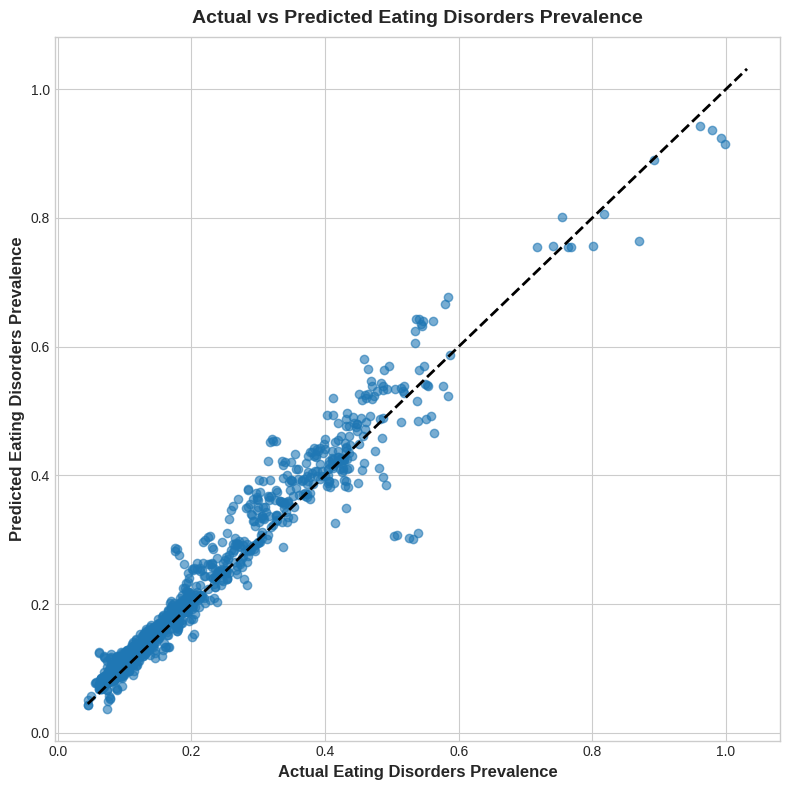
\includegraphics[scale=0.3]{figures/nn_predicted.png}
    %     \caption{Neural Network Predictions.}
    %     \label{fig:nn_pred}
    % \end{figure}
    % \begin{figure}[!ht]
    %     \centering
    %     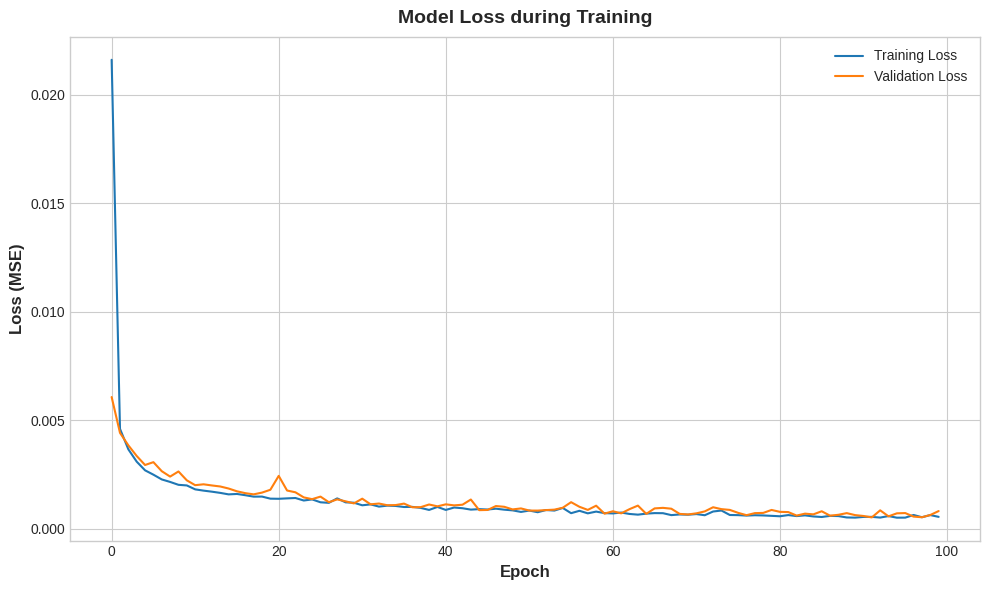
\includegraphics[scale=0.3]{figures/nn_model_loss.png}
    %     \caption{NN Model Loss.}
    %     \label{fig:nn_model_loss}
    % \end{figure}

\subsection{Random Forest Regressor}

The Random Forest Regressor is an ensemble learning algorithm that builds multiple decision trees and outputs the average of their predictions to estimate a continuous target variable. By averaging over many trees trained on different subsets of the data (via bootstrapping), it reduces overfitting and improves generalization. Unlike XGBoost, which builds trees sequentially and focuses on correcting errors made by previous trees, Random Forest builds trees independently in parallel. This simplicity comes with the benefit of easier interpretability and tuning, as its hyperparameters primarily control the number and depth of trees in the forest.

A simple analogy for describing the differences between decision trees (DT), random forests (RF) and XGBoost is playing a hole of golf: 
\begin{itemize}
    \item for DT you get one shot off the tee
    \item for RF you can hit many balls and pick the best one
    \item for XGBoost you can hit one ball walk up to the ball and hit it again until you get close to the hole as possible
\end{itemize}

    % \begin{figure}[!ht]
    %     \centering
    %     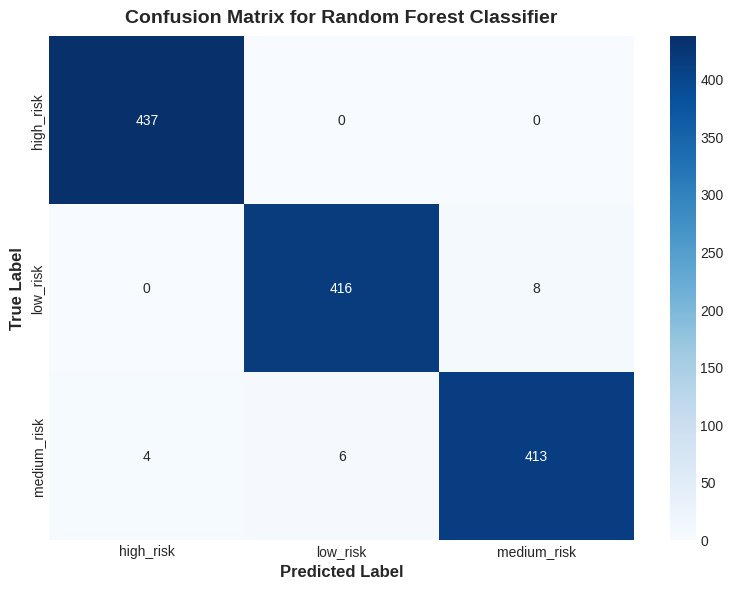
\includegraphics[scale=0.3]{figures/rnd_conf_matric.png}
    %     \caption{Random Forest Confusion Matrix.}
    %     \label{fig:rf_confusion_matrix}
    % \end{figure}
    % \begin{figure}[!ht]
    %     \centering
    %     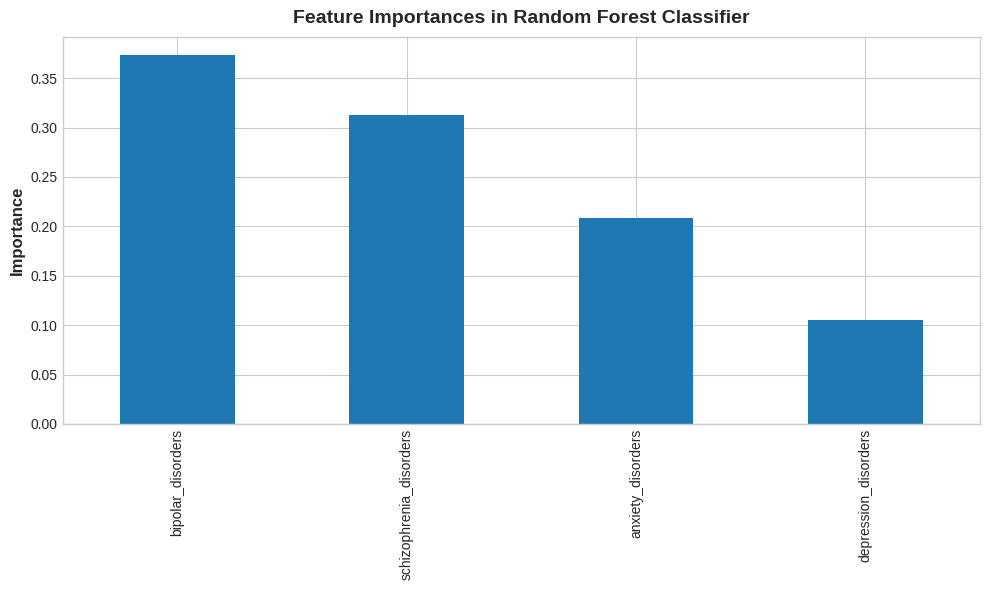
\includegraphics[scale=0.3]{figures/rnd_feature_importance.png}
    %     \caption{Random Forest Feature Importance}
    %     \label{fig:rf_importance}
    % \end{figure}
    % \begin{figure}[!ht]
    %     \centering
    %     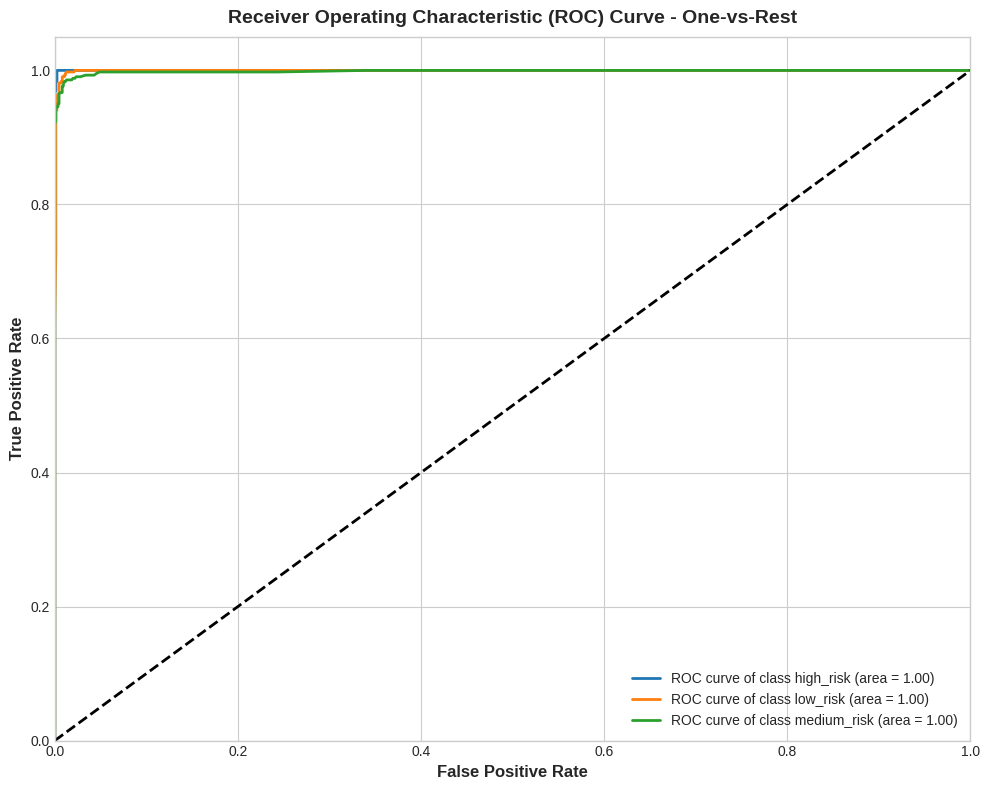
\includegraphics[scale=0.3]{figures/rnd_roc_curve.png}
    %     \caption{Random Forest ROC Curve.}
    %     \label{fig:rf_roc}
    % \end{figure}
    

\subsection{K-Nearest Neighbours}

K-Nearest Neighbours (KNN) is a supervised learning algorithm that predicts the output for a given data point by looking at the outputs of the K most similar instances in the training set. Similarity is typically measured using a distance metric like Euclidean distance. In regression, the predicted value is usually the average of the target values of these K neighbours. KNN is non-parametric, meaning it makes no assumptions about the underlying data distribution, and it can model complex relationships with sufficient data.

\begin{algorithm}
    \caption{K-Nearest Neighbours (KNN) Regression}
    \label{algo:knn}
    \begin{algorithmic}[1]
        \Require{$\mathbf{X} = \{x_1, x_2, \ldots, x_n\}$ (training features), $\mathbf{y} = \{y_1, y_2, \ldots, y_n\}$ (target values), $x_{\text{query}}$ (query point), $K$ (number of neighbours)}
        \Ensure{Predicted value $\hat{y}$ for $x_{\text{query}}$}
        \Statex
        \Function{KNNRegression}{$\mathbf{X}, \mathbf{y}, x_{\text{query}}, K$}
        \For{$i \gets 1$ to $n$}
            \State $d_i \gets \|x_i - x_{\text{query}}\|$
            \Comment Compute distance from query point
        \EndFor
        \State Identify indices $I$ of $K$ nearest neighbours with smallest $d_i$
        \State $\hat{y} \gets \frac{1}{K} \sum_{i \in I} y_i$
        \Comment Predict as average of $K$ nearest target values
        \State \Return $\hat{y}$
        \EndFunction
    \end{algorithmic}
\end{algorithm}

\subsection{Support Vector Regressor}

Support Vector Regression (SVR) is a supervised learning algorithm derived from Support Vector Machines (SVMs) (\cite{svr}), but designed for predicting continuous outcomes rather than classifying categories. In the context of predicting outcomes such as the severity or risk of eating disorders, SVR constructs a function that fits the data within a specified margin of tolerance, rather than attempting to classify it into discrete groups. The algorithm seeks a regression hyperplane that minimizes deviations beyond a pre-defined threshold (epsilon), while simultaneously ensuring that the model remains as flat (simple) as possible. The support vectors in this context are the data points that lie on or outside the margin and influence the position of the regression line \cite{kuhn2016}.

To capture complex, nonlinear relationships between features and the target variable, we apply the Radial Basis Function (RBF) kernel. This kernel function implicitly maps the input data into a higher-dimensional feature space, allowing the SVR model to learn nonlinear patterns without explicitly performing the transformation. This flexibility is especially useful when the input features have intricate interactions. To ensure the training and testing datasets maintain representative distributions, we use stratification during data splitting.
    